% ================================================================
% ================================================================
% --- PREAMBLE
% --- Document class
\documentclass[12pt]{article}

% --- Packages
\usepackage[utf8]{inputenc}
\usepackage[top=1in, bottom=1in, left=1in, right=1in]{geometry}
\usepackage{setspace}
\usepackage{microtype}
\usepackage[dvipsnames]{xcolor}
\usepackage{lastpage}
\usepackage{hyperref}
\usepackage{fancyhdr}
\usepackage{booktabs}
\usepackage{graphicx}
\usepackage{todonotes}
\usepackage{fontspec}
\usepackage{adjustbox}
\usepackage{float}
\usepackage{dcolumn}
\usepackage[backend=biber, style=apa, citestyle=apa]{biblatex}

% --- Settings
%\setmainfont{Caladea}
\usepackage{libertine}
\usepackage[libertine]{newtxmath}
\addbibresource{references.bib}

\hypersetup{
    colorlinks = true,
    linkcolor  = blue,
    urlcolor   = blue,
    citecolor  = blue,
    }
    
\pagestyle{fancy}

% --- Header and footer
\fancyhf{}
\headheight = 28pt
\chead{20 YEARS OF DOLLARIZATION IN ECUADOR\\
       \textit{Nicolás Cachanosky and John Ramseur}}
\cfoot{\footnotesize Page \thepage \hspace{0.5pt} of \pageref{LastPage}} 

% --- Title page
\title{20 YEARS OF DOLLARIZATION IN ECUADOR: A SYNTHETIC CONTROL ANALYSIS
       \thanks{We appreciate comments by Lawrence H. White. Any error or omission is our own.} \\
       \bigskip}

\author{
        \textbf{Nicolás Cachanosky} \\
        Metropolitan State University of Denver \\
        Department of Economics \\
        \href{mailto:ncachano@msudenver.edu}{ncachano@msudenver.edu} \\
        \and
        \textbf{John Ramseur} \\
        Metrpolitan State University of Denver \\
        Department of Economics \\
        \href{mailto:jramseur@msudenver.edu}{jramseur@msudenver.edu} \\
        \bigskip}

\date{\today}


% ================================================================
% ================================================================
% --- DOCUMENT
\setlength{\marginparwidth}{2cm}
\begin{document}


% ================================================================
% --- TITLE PAGE

\maketitle

\begin{abstract}
\noindent
This paper studies the 20-year experience of Ecuador's dollarization. It first reviews common concerns about about macroeconomic and financial stability under dollarization. It then applies a synthetic control analysis to Ecuador's economy. We find that Ecuador's monetary reform resulted in higher levels of income per capita, no clear effect on total factor productivity, a lower unemployment rate as well as a reduction in income distribution. Overall, results indicate that dollarization was beneficial for Ecuador.
\end{abstract}

\bigskip \bigskip
\footnotesize \noindent \textbf{JEL codes}: E42; E50; O43 \\
\footnotesize \noindent \textbf{Keywords}: Ecuador, dollarization, synthetic control analysis

\newpage
\doublespacing


% ================================================================
% --- SECTION 1: INTRODUCTION
\section{Introduction} 
    \label{sec:intro}

Dollarization was as topic of debate at the turn of the century. Not only because of the impact of international financial crisis such as the one one south east Asia or Russia, but also because of domestic problems in a number of emerging economies. For instance, Ecuador dollarized its economy in the year 2000 after an inflation crisis. Another Latin American country, Argentina, abandoned its currency board in a spectacular crisis in 2001 after rejecting the idea of dollarization. Even though the general interest on dollarization fade away as the 2000s moved forward, this monetary regime is gaining some relevance once again with the persisting high inflation rates in countries such as Argentina and Venezuela. Ecuador offers a twenty-year experience of dollarization that is valuable to inform on the pros and cons of this monetary regime.

Even though history offers more than hundred cases of dollarization \parencite{Schuler2005}, usable data for typical regression analysis remains a challenge. Data is limited, scattered across history, and mostly related to small economies that are highly sensitive to idiosyncratic shocks. A large part of the literature is either speculative, focused on narrow empirical results, or in very specific issues \parencite[for a sample see][]{Levy-Yeyati2002,Salvatore2003}. Of course, some regression analysis exists, such as that of Edwards and Magendzo \parencite{Edwards2006}. However, their study includes only small countries and covers the period 1970-1998, leaving Ecuador outside their sample. 

With respect to Ecuador's experience, some scholars have studied how dollarization affects seigniorage, fiscal policy, stock returns, and how feasible is to de-dollarized Ecuador \parencite{Lange2005, Jansen2007, MariDelCristo2016, JAMESON2003}. This paper offers the Nobel application of a synthetic control analysis (SCA) \parencite{Abadie,Abadie2003,Abadie2015} to the case of Ecuador's dollarization. This method builds a synthetic non-dollarized Ecuador that can be used as a counterfactual to evaluate the effect of dollarization. The ideal counterfactual is not what happened to Ecuador before and after dollarization, but how dollarized Ecuador compares to a non-dollarized Ecuador. SCA is useful because a real-world non-dollarized Ecuador is not observable. This method allows to evaluate the general impact of dollarization in a relative large-dollarized economy even if a full regression analysis is not feasible. We find that dollarized Ecuador outperforms the synthetic non-dollarized Ecuador in variables such as real GDP per capita, unemployment, and income distribution. We also find no significant impact on total factor productivity (TFP). Overall, we find that dollarization was beneficial for Ecuador.\footnote{In recent years, SCA has been applied in a number of different studies. For instance, Rok \parencite*{Spruk2019} studies the economic cost of institutional shocks to Argentina; Grier and Maynard \parencite*{Grier2016} and Absher, Grier, and Grier \parencite*{Absher2020} study market reforms in Georgia; and Powell, Clark, and Nowrasteh \parencite*{Powell2017} look at the impact of mass immigration in Israel.}

Some scholars consider dollarization to be an interesting reform to be considered by countries with troubled currencies \parencite{Avila2019,Cochrane2018,Gale2002,Hanke2003a,White2014a,Alesina2001,Mendoza2001}. Other scholars are critical of dollarization. Sachs and Larrain \parencite*{Sachs1999} offer a good representation of those who oppose to dollarization arguing that it is a "reckless" (p. 80) straitjacket. Ecuador's two-decade experience with dollarization offers a unique opportunity to be less speculative and more empirical about the real-world effects of dollarization.

The paper proceeds in the following way. Section 2 reviews how typical roles of a well-functioning central bank such as being a lender of last resort (LOLR) or how domestic monetary policy can be replaced under dollarization. Section 3 presents the SCA analysis and results. Section 4 concludes.


% ================================================================
% --- SECTION 2: HOW CAN DOLLARIZATION REPLACE TYPICAL ROLES OF A CENTRAL BANK
\section{How can Dollarization Replace Typical Roles of a Central Bank}
    \label{sec:debate}

Dollarization is the adoption of a foreign currency by a domestic country whether the currency adopted is the US dollar (USD), the New Zealand dollar, the Euro, the British Pound, or any other foreign currency. Dollarization can either by unilateral or bilateral. In the former case, the dollarizing country unilaterally decides to adopt a foreign currency. In the latter, there is an agreement with the foreign central bank that can include, for instance, sharing some of the new seigniorage that dollarization will produce. Dollarization can also be formal or informal. In the former case, the government formally adopts a foreign currency, while in the latter case economic agents decide to use a foreign currency regardless of the government's mandate. The distinction between formal and informal dollarization is important because it draws a distinction between a spontaneous and planned dollarization reforms. In the first case we have a bottom-up institutional change spontaneously driven by the private sector. In the second case we have a top-down government reform. Ecuador represents a bottom-up dollarization in the sense that it was the public who chose to use the USD and later on the government decided to formalize such decision \parencite{White2014a}. It was not the government who imposed the USD on the public, it was the public who imposed the USD on the government.\footnote{For a more detailed analysis of Ecuador's dollarization see Beckerman and Solimano \parencite*{Beckerman2002}.} Latin America is an example of a region with a number of countries informally dollarized.\footnote{Dollarization is similar but different to a currency union. Under a currency union monetary policy is decided by the member countries. In the case of dollarization, the dollarized economy has no say on how monetary policy is going to be executed by the foreign country.} 

It is useful to split the views on dollarization in two. The \textit{naive} view assumes that dollarization is a \textit{sufficient} reform to fix most of the issues in the domestic economy. On the other hand, the \textit{savvy} view takes the position that dollarization is a \textit{necessary} (even if not sufficient) reform needed to fix issues in the domestic economy. The naive version is a straw-man version of the savvy view and, therefore, the wrong target of criticism. Dollarization should be seen an a component of larger economic and institutional reform. Dollarization can help, for instance, to balance the budget by eliminating the possibility of monetizing deficits, but it cannot do it by itself. Ideally, dollarization is one piece of a larger reform.

There are four concerns with dollarization worth paying attention to: (1) the loss of domestic monetary policy, (2) the absence of a lender of last resort (LOLR), (3) the loss of seigniorage, and (4) because savvy dollarization requires other reforms such as a balanced budget, it seems that dollarization becomes unnecessary by its own necessary conditions. We discuss these four issues next and we point to how some of these problems are dealt with in dollarized economies such as Ecuador or Panamá.

% --- SUB-SECTION 2.1
\subsection{The Problem of Loosing Monetary Policy}

When a country dollarizes it gives up the possibility of executing its own domestic monetary policy. The possibility of executing monetary policy is particularly important in the presence of foreign nominal shocks that would require a prudent and well calibrated reaction by a domestic central bank. In other words, dollarization does not allow for a flexible exchange rate. Yet, the point of dollarization is precisely to eliminate domestic monetary policy. The reason for the odd argument that domestic monetary policy should be eliminated is that, in some extreme cases, domestic monetary policy proves to be worse than being exposed to foreign nominal shocks. A central bank can be a constant source of nominal shocks and high inflation rather than a source of monetary stability. It is important to keep in mind that dollarization is an issue in countries with extreme or long-lasting monetary imbalances. These are countries where a well-functioning and independent central bank is unfeasible regardless of how desirable it may be in the ideal.

A cost-benefit analysis of dollarization must avoid falling into a Nirvana-type fallacy \parencite{Demsetz1969}. The opportunity cost of dollarization is not a well-functioning central bank, it is the chronically inefficient monetary policy affecting the country that pushed the situation to the point where a potential dollarization becomes a reality. Countries that face a potential dollarization do not have an ideal central bank, they do not have more or less efficient central banks, they neither have inefficient central banks, they have \textit{very} inefficient central banks. The realistic choice is between dollarization and a central bank unable to commit to a minimum level of efficiency.

It is also unclear that in countries that face a potential dollarization domestic monetary policy is as independent from foreign policy as it is assumed to be. Monetary policy independence requires the adoption of a free floating exchange rate. However, many developing countries suffer from fear of floating or fear of appreciation \parencite{Calvo2002, Levy-Yeyati2003}, which means that in practice the domestic central bank is deviating from the ideal domestic strategy and, to some extent, following foreign monetary policy. If domestic monetary policy is going to be reticent to devalue or appreciate when facing foreign shocks, then it is unclear what benefit the domestic country is giving up by dollarizing. The degree of monetary independence that a central bank gives up when dollarizing is inversely related to its fear of depreciation or appreciation.

For the purpose of framing this discussion, assume the domestic central bank follows the following Taylor-rule reaction function.\footnote{This reaction function is presented just for illustration purposes. A country that faces a potential dollarization is in such monetary disorder that the central bank may not follow any reaction policy other than a day-to-day decision about how to make it to the next day.}

\begin{equation} \label{Eq:1}
    i_t = i^*_t + \phi_\pi \tilde{\pi}_t + \phi_X \tilde{X}_t + \varepsilon_t
\end{equation}

where $t$ is the time period, $i$ and $i^*$ denote short-term and short-term equilibrium interest rates respectively, $\tilde{\pi}$ is the inflation gap, $\tilde{X}$ is the gap of other feedback variables (such as the output or unemployment gap), $\phi$ are positive numbers and $\varepsilon$ is an error term that captures nominal shocks.

A deviation form the interest rate dictated by the policy rule would produce economic costs because of misallocation of resources, relative price distortion, monetary illusion, and so on. The larger (positive or negative) the value of $\varepsilon$, the larger the deviation form the ideal monetary policy. The concern is that a dollarized economy would be unable to adjust to a foreign nominal shock. However, we know from dollarization cases such as Ecuador that large deviations from the ideal monetary policy can also originate domestically. Far from being a settled issue, comparing the costs of domestic and external monetary shocks is an empirical question.

Consider the case of Ecuador, between 1983 and dollarization in 2000, the average yearly inflation rate was 42.2-percent. In 2000 the inflation peaked at 96-percent, by 2004 the inflation rate was below 3-percent. In terms of external large nominal shocks, Ecuador did not just faced the 2008 crisis, it also declared a default on its sovereign debt. Instead of falling into a large crisis, as would be expected from a nominal shock of the size of the 2008 crisis, real GDP per capita fell just 1.1-percent in 2009 starting to grow again next year. In comparison, Argentina's real GDP fell 6.9-percent in 2009 despite not being dollarized and having its own central bank. Argentina offers another example of a central bank as a source of domestic nominal shocks. Between the rise of Perón in 1946 and 2020, the yearly average inflation rate in Argentina is 62-percent. It is not clear that 74 years of an average inflation rate of 62-percent (which is also highly volatile) is better than dollarization. It could be objected that looking at Argentina's chronically troubled economy is unfair or unrepresentative. Yet, the point is to show that worse scenarios to that of dollarization are possible. Once this is accepted as a possibility, the option of dollarization can be treated more seriously than as a reckless idea.


% --- SUB-SECTION 2.2
\subsection{The Problem of the Absence of a Lender of Last Resort}

A dollarized economy does not have a central bank to perform the duties of a LOLR. This is problematic because the financial market is seen as inherently unstable. According to this view, illiquid banks are prone to suffer a bank run. If the bank run spreads through the financial market, then a LOLR is needed to get the situation under control and avoid a major financial crisis. For the purpose of this paper, we take the inherent instability of the banking sector as given.\footnote{The inherent instability view of banks rests on the Diamond and Dybvig \parencite*{Diamond1983} model. For a critical review of this model and its implications see Cachanosky \parencite*[][Ch. 1]{Cachanosky2018a}, Dowd \parencite*{Dowd1992a}, Selgin \parencite*[][Ch. 11]{Selgin1996c}, and White \parencite*[][Ch. 6]{White1999c}.}

Using Bagehot's rule as reference, a LOLR should lend at a premium rate only to illiquid but solvent banks. Moral hazard problems increase when a central bank deviates, or is expected to deviate, from this principle. As long as commercial banks expect the central bank to offer bailouts to insolvent banks, then banks in general will be inclined to invest in riskier assets increasing the likelihood of a financial crisis. To avoid moral hazard, a central banks adherence to Bagehot's rule must be credible. This credibility is not easy because central banks can bailout as many banks as desired without suffering losses or going bankrupt. It is also non-credible because of a time-inconsistency problem. While ex-ante it is optimal for a central bank to commit to a policy of financial discipline, ex-post a general bailout program may be preferable \parencite[][p. 469]{Gale2002}. Rational actors in the financial market understand this and the ultimate result can be excessive bailouts. In this context, dollarization can be interpreted as a credible commitment to not bailout banks when it should not be done at the cost of not being able to do so when needed \parencite{Gale2002}. When institutions are weak, the credibility of the central bank depends excessively in the personality of the president of the institution. If in addition central bank authorities have a quick turnaround, building durable credibility is not impossible. Between 1981 and 2000, the central bank of Ecuador had a total of eleven presidents (1.8 years in average). Another example is the central bank of Argentina, which bank had 23 presidents between 1983 and 2015 with an average of 570 days (1.56 years) in office. In situation liks this, the pressing question is not just how the central bank authorities think about monetary policy, but how much longer will they be in office.

However, a central bank is no the only form a LOLR can take and therefore dollarization should not be equated with total absence of a LOLR. Besides government alternatives to a central bank as a LOLR there are also market alternatives \parencite[][pp. 14-15]{Jacome2010}. Consider how this issue is handled in Ecuador, which is having a special tax on deposits that contributes to a liquidity fund that can be used if needed by a designated institution \parencite{Quispe-Agnoli2006}. This fund can be managed by a public office (as is the case of Ecuador) or by a consortium of private banks. The latter arrangement has stronger incentives to bailout only solvent banks than the former because their own resources are at risk (minimizing the likelihood of excessive bailouts). Another option is to mandate a deposit insurance.\footnote{The case of the United States is telling. Bank failures decreased with the implementation of the FDIC, not with the establishment of the Federal Reserve in 1913. See Selgin, Lastrapes, and White \parencite*[][pp. 582-583]{Selgin2012a}.} A third case would be to allow a deep financial integration with international markets as is the case of Panamá \parencite{MorenoVillalaz1999,MorenoVillalaz2005}. Banks operating domestically can be owned by foreign banks, who would have access to good quality financial information and also the incentive to keep their international branches in a good financial situation. There is also the option of regulating reserve requirements and credit diversification.  What is needed is an entity able to lend, not necessary one that can "print" its own money \parencite{Calvo2001}. In other words, a central bank is not only one of many LOLR arrangements, it may not even be the best alternative.

In addition, the capacity of a domestic central bank who serves as LOLR should not be overstated. Countries that face a potential dollarization do not have a high demand of their domestic currency. The run is not against banks, it is against the domestic currency (which happens to be deposited in banks). The domestic central bank cannot "print" foreign currencies, and therefore there is only so much it can do to stop a bank run. Supplying the required pesos does not stop the run against the bank, it rather fuels a financial crisis as the devalued currency finds its way to the exchange rate market. In this situation the domestic central bank needs access to foreign currency, not just to its own "printing press".

The more private-market oriented a LOLR is, the closer it should be expected to adhere to Bagehot's rule and minimize moral hazard problems and the likelihood of excessive bailouts. A privately managed fund risks loosing its resources if it saves banks that are insolvent, but a central bank doe not face the same cost-benefit incentives. The underlying issue in the case of dollarization is not whether or not there will LOLR services, but what type of LOLR should be in place. One that operates under the scope of government incentives in a country with weak institutions and monetary instability, or one that operates under the scope of market incentives.\footnote{Bagehot's rule was endorsed by Ben Bernanke when serving as Chairman of the Federal Reserve. It is less clear that the acts of the Fed followed this endorsement \parencite{Hogan2015b}.}

% --- SUB-SECTION 2.3
\subsection{The Problem of Lost Seigniorage}

Seigniorage is typically defined as the revenue accruing to the currency issuer. Under dollarization there is no seigniorage, at least in principle. It is common in the literature to not pay much attention to the distinction between seigniorage and the inflation tax. Some authors include the inflation tax as part of seigniorage, others do not include the inflation tax as part of proper seigniorage.\footnote{For instance, compare Easterly \parencite*[][fn. 1]{Easterly1995} and Hinds \parencite*[][ch. 6]{Hinds2006a}}. The difference, however, is relevant when studying a country considering a dollarization reform. For the purpose of this paper, I am using the latter distinction; seigniorage is the profit of the \textit{central bank} (the currency issuer) from its business operations of producing and selling fiat money, while the inflation tax is the purchasing power seized by the \textit{treasury} when monetizing the deficit. In a well functioning economy, seigniorage is larger than the inflation tax. Differently, a country facing a potential dollarization may have negative seigniorage while collecting a significant inflation tax.\footnote{For a discussion on different ways to measure seigniorage and the validity of implied assumptions when measuring seigniorage see Klein and Neumann \parencite*{Klein1990}.}

The central bank's revenue is the interest collected by investing foreign-denominated currency. As long as its fiat currency is demanded by the market, the central bank can create its currency, trade it in the market, and buy financial assets denominated in a world-reserve currency. The costs of the central bank are the interest rate it must pay for the market to hold its currency (for instance, issuing interest-bearing bonds) and its operational costs. The central bank can transfer some or all of the seigniorage to the treasury; then seigniorage will be part of the treasury's revenue. The central bank's seigniorage can be represented as follows (\ref{Eq:2}):

\begin{equation}\label{Eq:2}
    S = ei^FA - iB - C
\end{equation}

where $S$ is the central bank seigniorage, $e$ is the nominal exchange rate, $i^F$ is the foreign nominal interest rate, $A$ is the amount of foreign assets, $i$ is the domestic interest rate paid by the central bank, $B$ is the amount of bonds issued by the central bank, and $C$ denote the operational costs of the monetary authority.

If there is high inflation, then the low demand for the domestic currency means the central bank must pay a high value of $iB$, potentially producing a negative seigniorage. The more informally dollarized an economy is, and the higher the inflation rate is, the less seigniorage the government collects. Also, the higher the expected rate of depreciation is, the higher the domestic interest rate the domestic central bank must offer.\footnote{Let $\Delta$ denote change. Then: $S = ei^FA - (i^F + E[\Delta e / e])B - C$. Depreciation expectations reduce the amount of seigniorage. This can be a relevant issue in countries that let their currencies appreciate due to fear of floating.}

A dollarizing economy resigns more to the inflation tax than it does to seigniorage. The inflation tax is typically regressive and highly distorting. Also, as a non-legislated tax, it can be at odds with constitutional mandates. High inflation is not only economically costly, it can also contribute to institutional degradation. For a country facing an out of control inflation, giving up potential seigniorage may be a low price to pay to get monetary stability and getting rid of the distorting inflationary tax.

Yet, there is a way to maintain some seigniorage under dollarization. Following the examples of Scotland, Ireland and Hong Kong, domestic banks can be allowed to issue their own convertible banknotes \parencite[see][]{Hogan2012}. Different to the case of the central bank, in this situation seigniorage will be collected by the private sector rather than the government. A stronger reform, to be considered in countries with weak property rights protection to private deposits, would be to implement an off-shore banking regime as recommended by Ávila  \parencite*{Avila2019}.

% --- SUB-SECTION 2.4
\subsection{The Problem of Unnecessary Dollarization by its Necessary Conditions}

The \textit{savvy} view of dollarization we mentioned before does not expect this monetary reform to solve all of the economic problems of a country. Other reforms such as balancing the budget, deregulate the labor market, or removing trade restrictions are some examples of other initiatives a country in need of dollarization should do (see \parencite[][pp. 17-20]{Jacome2010}). If all these other reforms are carried out, why dollarize? Seems that the necessary reforms to make dollarization robust and useful also makes it unnecessary.

Dollarization can still be useful in two ways. The first one is by being the trigger that makes other reforms happen. Dollarization may be unneeded if other reforms take place, but these other reforms may not take place without dollarization. The second one requires to avoid again a Nirvana-type fallacy of argument. Certainly, if the feasible reforms are the ideal ones, dollarization would not be needed. Yet, the feasible but realistic reforms may be enough for dollarization to work even if they are not ideal. In that case, dollarization works as an institutional constrain on the government. Dollarization is not just a monetary policy reform, it is also an institutional reform that is very costly to revert because it is not easy to launch a new fiat currency \parencite[see]{Selgin1994b}. Dollarization is not only a monetary policy reform, it is also a non-reversible institutional reform.

Figure \ref{fig:Fig01} assumes that institutional quality ranks from 0 (worse) to 100 (best or ideal). Assume further that the institutional quality of a country considering dollarization is 40. Dollarization needs an institutional quality of 70 to be sustainable and beneficial, and becomes unnecessary with an institutional quality of at least 90. The realistic institutional reform this country can produce would give an institutional quality of 80; more than what is necessary for dollarization to work, less than what would make it unnecessary.

\begin{figure}[!htbp]
    \caption{Institutional reform and dollarization}
    \centering
    \includegraphics{Figures/Fig_01.png}
    \label{fig:Fig01}
\end{figure}

The institutional robustness of dollarization should not be underestimated. Dollarization in Ecuador survived (1) the left-leaning populist regime of Rafael Correa, (2) a sovereign debt default, and (3) the 2008 financial crisis. Arguably, dollarization served as a constrain on populist policies. Absher, Grier, and Grier \parencite*{Absher2020} find that durable left-populist regimes in Latin America produce significant losses in real income. The only exception in their study is Ecuador, which is also the only dollarized country in their sample. This result suggests that dollarization may work as an institutional constraint against populist regimes.\footnote{On populism and institutions see Abts and Rummens \parencite*{Abts2007}, Cachanosky, Padilla, and Gómez \parencite*{Cachanosky2021b}, de la Torre \parencite*{DelaTorre2017}, Mazzuca \parencite*{Mazzuca2013},  Riker \parencite*{Riker1988}, and Rode and Revuelta \parencite*{Rode2015}.} Using the Economic Freedom of the World Index (EFW) as a proxy of institutional quality, Ecuador ranks 118 out of 162 countries (73 percentile), just below Guyana and above Vietnam \parencite{EFW_2019}. This result shows that Ecuador did not have to become one of the freest economies in the world to have a durable dollarization. Ecuador is a case where the institutional reforms were enough for dollarization to survive for two decades even if they are not good enough to make dollarization unnecessary. It also suggests that any shortcoming in Ecuador's economy should not be automatically put on dollarization when there is still plenty of room for further institutional reforms.


% ================================================================
% --- SECTION 3: SYNTHETIC CONTROL ANALYSIS
\section{Synthetic Control Analysis}
    \label{sec:SCA}

\subsection{The SCA Method and Donor Pool Selection Criteria}

SCA allows to build a counterfactual, non-dollarized Ecuador, and compare the evolution of key economic variables such as GDP per capita, TFP, unemployment, and income distribution (GINI coefficient) with real-world dollarized Ecuador. This method allows to deal with fixed effects interacting with time-varying coefficients when there is only one treated unit (in our case Ecuador). In simpler terms, synthetic Ecuador is built as a weighted average of countries included in a donor pool.

A few requirements are needed for a proper application of the SCA method. First, the donor pool must include countries that share similar characteristic to the treated unit. SCA prioritizes a representative donor pool over a large-as-possible sample. A larger sample may include non-representative countries that can reduce the efficiency of the estimation or produce overfitting. In SCA, more data is not always better. Second, the treated country must be the only one in the sample being affected by the shock under analysis and the shock must occur at a definite point of time. Ecuador must be the only country going through dollarization. Third, there should be enough observations in the pre-shock period for the SCA to be able to build a credible synthetic Ecuador.

Besides the donor countries, a number of covariates (predictor) variables are chosen as well (see table \ref{table:sources}). The SCA method minimizes the root-mean-squared-prediction-error (MSPE) of the average of the covariates in the pre-shock period. To do so, SCA assigns relative weights to each covariate depending how good they are in predicting the outcome variable. These relative weights are captured in a diagonal matrix (the V matrix). The diagonal values of the V matrix are non negative and normalized to one. Therefore, covariates with low explanatory power over the outcome variable have low values in the V matrix. \footnote{More formally, let there be $j = 1,...,J$ countries in the donor pool and $W$ be a vector of non-negative weights assigned to each country $(w_j \geq 0)$. Then, SCA estimates $W^*$ such that $W^* = \operatorname{arg\min} (X_1 - X_0W)'V(X_1 - X_0W)$ where $X_1$ contains the covariates from the treated country and $X_0$ contains the covariates it the donor countries. $V$ is a diagonal matrix with non-negative components.}

Our donor pool is limited to Latin America countries to maintain an overall social and economic similarity with Ecuador. The reason to limit our donor pool to Latin America is to avoid the accidental inclusion of a country that is not representative enough of Ecuador social and economic characteristics. We also exclude Latin American countries that are dollarized such as Panamá and El Salvador.\footnote{We do include Argentina, which was under a currency board during the 1990s. However, Argentine had an heterodox currency board which allows deviations from its strict (orthodox) adherence \parencite{Hanke2008}.} The donor countries are: (1) Argentina, (2) Bolivia, (3) Brazil, (4) Chile, (5) Colombia, (6) Costa Rica, (7) Mexico, (8) Paraguay, (9) Perú, and (10) Uruguay

\begin{table}[!htbp]
\begin{center}
\caption{Data source and summary statistics} \label{table:1}
\begin{tabular}{lccl} \\ \toprule
  Variable                   & Mean  & Std. Dev. & Source                     \\ \midrule
  \textbf{Predicted}         &       &           &                            \\
  GDP per Capita (PPP, 2017) & 9,188 & 4,558     & The Maddison Project       \\
  TFP (PWT) (2017=1)         & 0.98  & 0.11      & Penn World Tables          \\
  TFP (CB) (\% change)       & -0.66 & 2.85      & The Conference Board       \\
  Unemployment rate          & 7.48  & 3.68      & World Bank (WDI)           \\
  GINI coefficient           & 46.10 & 4.38      & World Bank (WDI) and SWIID \\ \midrule
  \textbf{Predictors}        &       &           &                            \\
  Industry (\% of GDP)       & 30.10 & 5.22      & World Bank (WDI)           \\
  Manufacturing (\% of GDP)  & 17.12 & 4.69      & World Bank (WDI)           \\
  Investment (\% of GDP)     & 18.69 & 4.36      & World Bank (WDI)           \\
  Trade openness             & 48.08 & 20.85     & World Bank (WDI)           \\
  FDI (\% of GDP)            & 2.57  & 2.35      & World Bank (WDI)           \\
  Labor                      & 0.49  & 0.07      & World Bank (WDI)           \\
  Gross capital formation    & 0.19  & 0.04      & World Bank (WDI)           \\
  Human Capital Index        & 2.39  & 0.33      & World Bank (WDI)           \\
  Urban (\% of total)        & 72.19 & 13.71     & World Bank (WDI)           \\ \bottomrule 
\end{tabular}
\end{center}
\end{table}

Using all pre-treatment values of the outcome variable to predict its post-treatment values can lead to inaccurate results or bias \parencite{Ashok2015}. Therefore, we offer two models for each SCA estimation. Both models share the same covariates, but model 1 also includes selected observations in the pre-treatment period of the outcome variable. We use this approach for all SCA estimations below. Table \ref{table:countries} shows the country weight for each outcome variable and for each SCA model.

\begin{table}[!htbp]
\begin{center}
\caption{Country weights per outcome variable and SCA model} \label{table:countries}
\begin{tabular}{l c c c c c c c c} \\ \toprule
  & \multicolumn{2}{c}{GDP per capita (PPP)} & \multicolumn{2}{c}{TFP} & \multicolumn{2}{c}{Unemployment} & \multicolumn{2}{c}{GINI}                \\ 
  Country    & SCA 1 & SCA 2 & SCA 1 & SCA 2 & SCA 1 & SCA 2 & SCA 1 & SCA 2 \\ \midrule
  Argentina  &       &       &  35.8 &  11.7 &       &       &       &       \\
  Bolivia    &  64.6 &       &       &   0.4 &   7.9 &       &       &       \\
  Brazil     &       &       &       &   0.2 &  44.3 &  56.1 &       &       \\
  Chile      &       &       &       &   3.8 &       &       &       &  17.1 \\
  Colombia   &       &       &       &   0.4 &  44.9 &       &       &       \\
  Costa Rica &       &       &       &   0.8 &       &       &  18.8 &   6.4 \\
  Mexico     &  35.4 &  20.5 &  21.3 &  70.8 &       &       &   5.0 &       \\
  Paraguay   &       &  72.8 &  41.0 &   9.2 &       &   7.3 &  37.7 &  76.5 \\
  Perú       &       &   6.7 &   1.9 &   0.8 &   3.8 &  36.6 &  38.6 &       \\
  Uruguay    &       &       &       &   2.0 &       &       &       &       \\
  \bottomrule 
\end{tabular}
\end{center}
\end{table}

\subsection{Real GDP per Capita (PPP)}

Our first estimation is real GDP per capita (PPP adjusted).\footnote{It is common in the SCA literature to use PPP adjusted real GDP per capita. See, for instance, Abadie, Diamond, and Hainmuller \parencite*{Abadie2015}, Absher, Grier, and Grier \parencite*{Absher2020}, Cavallo, Noy, and Pantano \parencite*{Cavallo2013}, Campis, Coricelli, and Moretti \parencite*{Campos2019}, and Lawson, Grier, and Absher \parencite*{Lawson2019}.} Consider that dollarization occurs at the same time that price of commodities start to rise in the early 2000s. It is expected to observe an upward trend in Ecuador's income per capita with or without dollarization. Ecuador's rise in GDP per capita (PPP) exemplifies the difficulty of evaluating dollarization as a before-and-after comparison. Dollarization is beneficial if GDP per capita (PPP) rises \textit{more} that it would have done so without the dollarization reform.  

Table \ref{table:GDP_balance} shows the predictor balance (how well synthetic average variables match treatment's average variables), V matrix values, and RMSPE for both SCA models. With the given sample, two or three countries are needed to minimize the RMSPE of synthetic Ecuador. The tables show that the model that includes two observations of the outcome variable has a lower RMSPE but the outcome values carry most of the weight as explanatory values.

\begin{table}[!htbp]
\begin{center}
\caption{SCA for GDP per Capita (PPP), predictor balance and V matrix} \label{table:GDP_balance}
\begin{tabular}{l r r r r r r}     \\ \toprule
  Variable                    &    Ecuador &  Synthetic 1 & V matrix 1 & Synthetic 2 & V matrix 2 \\ \midrule 
  Industry (\% GDP)           &      28.41 &        29.79 &     0.0163 &       28.88 &     0.4592 \\
  Manufacturing (\% GDP)      &      21.35 &        16.65 &     0.0131 &       15.80 &     0.0064 \\
  Investment (\% GDP)         &      21.15 &        14.30 &     0.0005 &       19.87 &     0.5262 \\
  Unemployment rate           &       8.53 &         7.39 &     0.0001 &        5.47 &     0.0083 \\ \midrule
  GDP per capita (PPP) (1981) & \$5,831.00 &   \$5,627.20 &     0.6631 &             &            \\
  GDP per capita (PPP) (1999) & \$4,797.00 &   \$5,621.58 &     0.3070 &             &            \\ \midrule
  RMSPE                       &            &       315.62 &            &      375.11 &            \\
  \bottomrule 
\end{tabular}
\end{center}
\end{table}




Figure \ref{fig:SCA_GDP} depicts dollarized Ecuador along both SCA estimations. As expected, we see the three lines starting an upward trend at the same time the price of commodities start to rise in the early 2000s. However, GDP per capita (PPP) outperforms both SCA estimations; real income of Ecuador adjusted by cost of living grew more than it would have absent the dollarization reform. The plot also depicts the impact of the 2008 crisis. Despite being dollarized, Ecuador's real GDP (PPP) remained higher than the non-dollarized counterfactual estimations. And, as mentioned above, real GDP per capita (PPP) in Ecuador fell less than in non-dollarized countries such as Argentina.

\begin{figure}[!h]
    \caption{SCA: Real GDP per capita (PPP)}
    \centering
    \includegraphics{STATA/Fig_GDP_SCA.pdf}
    \label{fig:SCA_GDP}
\end{figure}

The plot also shows that starting in 2015 Ecuador's real GDP (PPP) falls and then stagnates in 2016. This does not occur in the counterfactual, which may suggest that the issue rests on Eucador's use of a foreign currency. However, the reason for this change in trend is a combination of (1) fall in oil prices, (2) increased tax on exports, and (3) the 2016 earthquake. In particular the latter is a real shock absent in the donor countries that build the synthetic Ecuador. These new shocks mean that dollarization is not the obvious reason of the change in real income and that the later years of the SCA method should be read with care. The longer the time after the shock is included in the SCA, the more likely a new set of shocks will affect the SCA comparison.

The spread between dollarized Ecuador and its synthetic estimations is economically significant. By 2005, Ecuador is producing a 5-percent higher real income (PPP adjusted), by 2010 Ecuador is producing between 8-percent and 11-percent higher than the synthetic estimations (figure \ref{fig:SCA_gap}). At the peak, dollarization brought between 12-percent and 20-percent of higher PPP adjusted per capita real income. In terms of real income, it is plausible that monetary stability and credible reforms brought more benefits to Ecuador's economy than being undefended from foreign shocks (recall that Ecuador still has a liquidity fund at its disposal).

\begin{figure}[!h]
    \caption{SCA: Real GDP per capita (PPP) synthetic gap}
    \centering
    \includegraphics{STATA/Fig_GDP_GAP.pdf}
    \label{fig:SCA_gap}
\end{figure}

\subsection{Total Factor Productivity}

Similar to GDP, we use PPP adjusted growth rates of GDP. While TFP growth rates are small in magnitude, they do depict opposite signs between dollarized and synthetic Ecuador. Post-dollarization, Ecuador has a 0.14-percent average annual growth rate of TFP, while synthetic estimations result in  negative 0.02-percent and negative 0.35-percent annual average growth for both model estimations respectively. 

We show first the predictor balance and V matrix for each SCA model. Even though values from the outcome variable have very low V matrix values, its RMSPE is lower than the model when not using outcome values as predictors. Figure \ref{fig:SCA_TFP} depicts the SCA results. Consider three points in the plot. The first one is the quicker recovery of TFP growth rates immediately after the dollarization reform which does not occur in either synthetic estimation. The second is the nominal shock of the 2008 crisis, Ecuador's TFP falls less than the non-dollarized counterfactuals. The third one is, again, the slow down of the economy starting in 2014. As discussed in the previous section, this is due to a new set of shocks affecting Ecuador's economy but not the donor pool.

\begin{table}[!htbp]
\begin{center}
\caption{SCA for TFP (PPP and in real terms), predictor balance, V matrix, and RMSPE} \label{table:TFP_balance}
\begin{tabular}{l r r r r r r}     \\ \toprule
  Variable                    &    Ecuador &  Synthetic 1 & V matrix 1 & Synthetic 2 & V matrix 2 \\ \midrule 
  Investment (\% GDP)         &     19.31  &       18.30  &       0.00 &      19.33  &       0.28 \\
  Trade openness              &     44.93  &       57.24  &       0.00 &      44.99  &       0.21 \\ 
  FDI (\% GDP)                &      2.06  &        2.06  &      ~1.00 &       2.06  &       0.23 \\
  HCI                         &      2.32  &        2.32  &       0.00 &       2.32  &       0.28 \\
  Labor compensation (\% GDP) &     37.00  &       44.86  &      ~0.00 &      42.28  &       0.00 \\ \midrule
  TFP (1995)                  &     -0.93  &       -1.22  &      ~0.00 &             &            \\
  TFP (1999)                  &     -3.23  &       -3.52  &       0.00 &             &            \\ \midrule
  RMSPE                       &            &        1.10  &            &       2.15  &            \\
  \bottomrule 
\end{tabular}
\end{center}
\end{table}

\begin{figure}[!h]
    \caption{SCA: TFP (constant prices and PPP adjusted)}
    \centering
    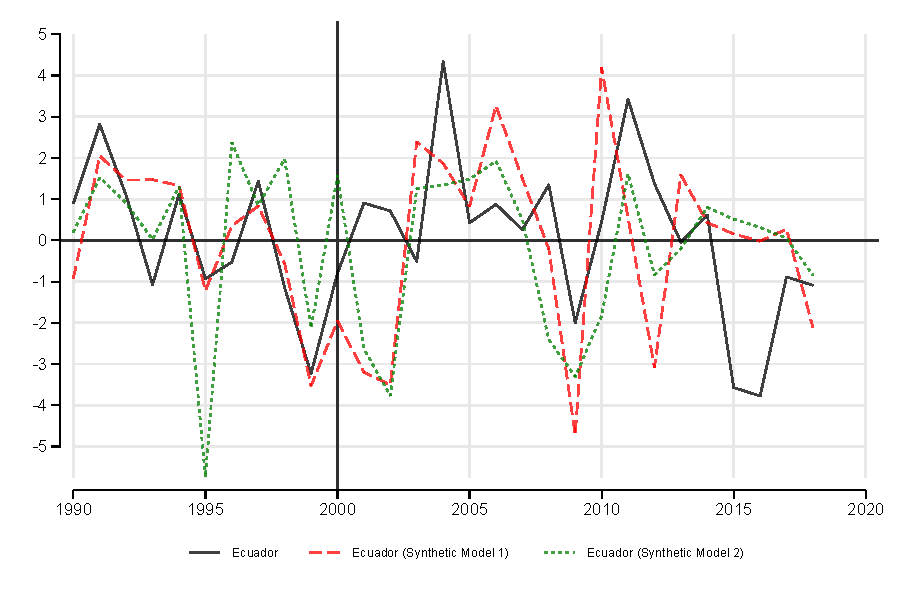
\includegraphics{STATA/Fig_TFP3_SCA.pdf}
    \label{fig:SCA_TFP}
\end{figure}

It is likely that Ecuador needs more regulatory reforms in order to benefit from higher TFP growth rates. Recall that Ecuador ranks low in the EFW index and that dollarization is not a sufficient, even if it is a necessary, reform to improve the economic performance of the dollarized economy. Nor surprisingly, after dollarization Ecuador's EFW score improved the most in the area of sound money. We use EFW as a useful proxy on the role of institutions and economic growth because a large body of the literature has found that EFW correlates with positive outcomes with almost no negative tradeoffs \parencite{Hall2014}. In particular, there is room for de-regulation in the labor market, the independence of the legal system, the protection of property rights, and the removal of non-tariff trade barriers. 

In terms of TFP volatility, which could translate to real business cycle movements, there is no clear difference in dollarized Ecuador with its synthetic counterfactual. The post-dollarization TFP standard deviation of the growth rate of TFP in Ecuador is 2-percent. SCA model 1 and 2 have a standard deviation of the growth rate of TFP of 2.5-percent and 1.58-percent respectively.

\subsection{Unemployment}

We now turn to the unemployment rate. Between 1990 and 2000, the unemployment rate depicts an upward trend, going from a low of 6-percent to a peak of 14-percent in 1999. After dollarization, the unemployment rate falls to 5-percent and enters what looks to be a slight downward trend. The most recent data for the unemployment rate is below 4-percent. 

Table \ref{table:UNEMP_balance} shows the predictor balance, V matrix values, and RMSPE for each estimation. SCA results are shown in figure \ref{fig:SCA_UNEMP}. Note that in this case SCA models 1 and 2 rely heavily on the unemployment rate of 1999 and FDI (\% GDP) respectively. Both estimations show that dollarized Ecuador has a persistent lower unemployment rate than the synthetic alternatives. It also shows a more stable unemployment rate starting in 2014. Despite its incomplete reforms in the labor market, dollarization correlates with a lower unemployment rate should Ecuador have kept its own central bank.

\begin{table}[!h]
\begin{center}
\caption{SCA for Unemployment rate, predictor balance, V matrix, and RMSPE} \label{table:UNEMP_balance}
\begin{tabular}{l r r r r r r}     \\ \toprule
  Variable                 &    Ecuador &  Synthetic 1 & V matrix 1 & Synthetic 2 & V matrix 2 \\ \midrule 
  GDP per capita (PPP)     &  \$4,952.3 &   \$6,811.32 &     0.0000 &  \$6,063.63 &     0.0000 \\
  Industry (\% GDP)        &      28.44 &        28.54 &     0.0000 &       28.41 &     0.0019 \\
  Trade openness           &      44.93 &        28.37 &     0.0000 &       27.04 &     0.0000 \\
  FDI (\% GDP)             &       2.06 &         2.08 &     0.0001 &        2.06 &     0.9981 \\ \midrule
  Unemployment rate (1990) &       5.88 &         7.02 &     0.0000 &             &            \\
  Unemployment rate (1999) &      13.96 &        13.96 &     0.9998 &             &            \\ \midrule
  RMSPE                    &            &         0.75 &            &        2.25 &            \\
  \bottomrule 
\end{tabular}
\end{center}
\end{table}

\begin{figure}[!h]
    \caption{SCA: Unemployment rate}
    \centering
    \includegraphics{STATA/Fig_UNEMP_SCA.pdf}
    \label{fig:SCA_UNEMP}
\end{figure}

Despite its incomplete reforms in the labor market, dollarization correlates with a lower unemployment rate should Ecuador have kept its own central bank. In addition, real minimum wages increases after dollarization favored labor substitution with capital \parencite{Soto2009}. A deregulated labor market without price controls would likely produce a more dynamic and flexible labor market. Concerns about employment levels should keep a SCA counterfactual in mind and do not overlook frictions produced by inefficient labor regulation.

\subsection{GINI coefficient}

Finally, we look at the case of income distribution as measured by the GINI coefficient (0: perfect equality; 100: perfect inequality). Results show that income distribution becomes more equal in dollarized Ecuador than it does in both non-dollarized synthetic estimations. The rise in income per capita has a larger effect on low-income population than it does on high-income population. The specific mechanics of how and why this occurs would be interesting research question to extend analysis of dollarization. As an example, a good candidate to explain a fall in the GINI coefficient would be a better financial integration and protection to low-income population. It is to be be expected that high-income individuals have the means to protect themselves against inflation.

\begin{table}[!h]
\begin{center}
\caption{SCA for GINI coefficient, predictor balance, V matrix, and RMSPE} \label{table:GINI_balance}
\begin{tabular}{l r r r r r r}     \\ \toprule
  Variable              &    Ecuador &  Synthetic 1 & V matrix 1 & Synthetic 2 & V matrix 2 \\
  \midrule 
  FDI (\% GDP)          &       2.06 &         2.52 &     0.0707 &        2.26 &     0.0000 \\
  Urban population (\%) &      57.49 &        60.65 &     0.1358 &       57.50 &     0.4076 \\
  Investment (\% GDP)   &      19.31 &        18.79 &     0.0000 &       19.31 &     0.5924 \\
  Human Capital Index   &       2.32 &         2.26 &     0.0719 &        2.20 &     0.0000 \\
  \midrule
  GINI (1992)           &      48.75 &        47.94 &     0.3075 &             &            \\
  GINI (1995)           &      49.01 &        49.68 &     0.4142 &             &            \\
  \midrule
  RMSPE                 &            &         0.45 &            &        1.41 &            \\
  \bottomrule 
\end{tabular}
\end{center}
\end{table}

\begin{figure}[!h]
    \caption{SCA: GINI coefficient}
    \centering
    \includegraphics{STATA/Fig_GINI_SCA.pdf}
    \label{fig:GINI}
\end{figure}

\begin{table}[!h]
\begin{center}
\caption{GINI coefficient, period average and change (2000 - 2017)} \label{table:GINI_summary}
\begin{tabular}{l r r r r}     \\ \toprule
  Country    & Period average & GINI (2000) & GINI (2017) & Difference  \\ \midrule 
  Argentina  &           41.7 &        45.7 &        37.5 &        -8.2 \\
  Brazil     &           47.9 &        52.0 &        45.9 &        -6.1 \\
  Chile      &           45.9 &        48.5 &        44.0 &        -4.5 \\
  Colombia   &           49.8 &        51.7 &        46.1 &        -5.6 \\
  Costa Rica &           45.3 &        44.1 &        45.9 &         1.8 \\
  Ecuador    &           45.6 &        49.7 &        41.9 &        -7.8 \\
  Mexico     &           44.7 &        47.3 &        41.7 &        -5.6 \\
  Paraguay   &           46.9 &        49.8 &        44.7 &        -5.1 \\
  Perú       &           48.1 &        51.5 &        44.3 &        -7.4 \\
  Uruguay    &           39.2 &        40.0 &        35.9 &        -4.1 \\
  \bottomrule 
\end{tabular}
\end{center}
\end{table}

GINI coefficient in post-dollarization Ecuador is at similar levels than the region. It is also one of the countries in the sample with the largest fall in the GINI coefficient (table \ref{table:GINI_summary}). Typically, a fall (rise) in the GINI coefficient is considered to be good (bad) even if the optimal (or fair) level of the GINI coefficient goes undefined. A \textit{perfect} income distribution as measured by the GINI construct may or may not be the \textit{optimal} or \textit{most fair} income distribution. Yet, according to the typical classification (lower values are always better) SCA analysis indicates the income distribution situation improved in Ecuador with dollarization with respect to the synthetic counterfactuals.


% ================================================================
% --- SECTION 4: CONCLUSIONS
\section{Conclusions}

Most cases of dollarization are found in small economies such as the Marshall Islands, Panama, Puerto Rico, San Marino, Lichtenstein, or Luxembourg. Dollarization in larger economies such as that of Ecuador are more rare. Ecuador does not only offer a case of a larger dollarized economy, it also offers a durable reform that survived the 2008 crisis, a sovereign debt default, and a left-leaning populist regime. In addition, it also offers a case where market friendly reforms are still lacking. 

Our SCA application looks at overall economic and social variables of interest such as income per capita (adjusted by cost of living), productivity, unemployment and income distribution. Overall, SCA indicates that Ecuador gain both, economically and socially with dollarization. Economic gains did not come at the expense of worse social indicators (or the other way around). Given that typical roles of a domestic central bank can be substituted in a dollarized economy (section \ref{sec:debate}), positive economic and social results are possible and theoretical-based concerns can, and should, be contrasted with real world experience.

Finally, the implications of dollarization reach beyond economic performance. As we suggest, a non-reversible monetary reform as dollarization can also provide an institutional shield against governments with authoritarian inclinations. The Ecuador case should also be of interest to the recent literature on the rise of the twenty-first century populism.


% ================================================================
% --- SECTION 5: REFERENCES
\newpage
\singlespacing
\printbibliography


% ================================================================
% --- THE END
\end{document}
